\begin{frame}[c]
    \begin{columns}[onlytextwidth]
    \begin{column}{0.55\textwidth}
    \textbf{Neutrino observatories}
        \begin{itemize}
            \item Usage in the \textbf{IceCube} simulation chain
            \begin{itemize}
                \item[$\rightarrow$] PROPOSAL provides the energy losses of muons and taus along the particle track
                \item[$\rightarrow$] Estimation of background contamination, e.g. due to undetected muons in veto regions
            \end{itemize}
            \item Usage in \textbf{NuRadioMC}, a framework for radio neutrino simulations
            \begin{itemize}
                \item[$\rightarrow$] Estimation of radio contribution due to muon and tau energy losses in ice
            \end{itemize}
        \end{itemize}
    \end{column}
        \begin{column}{0.45\textwidth}
            \begin{figure}
                \centering
                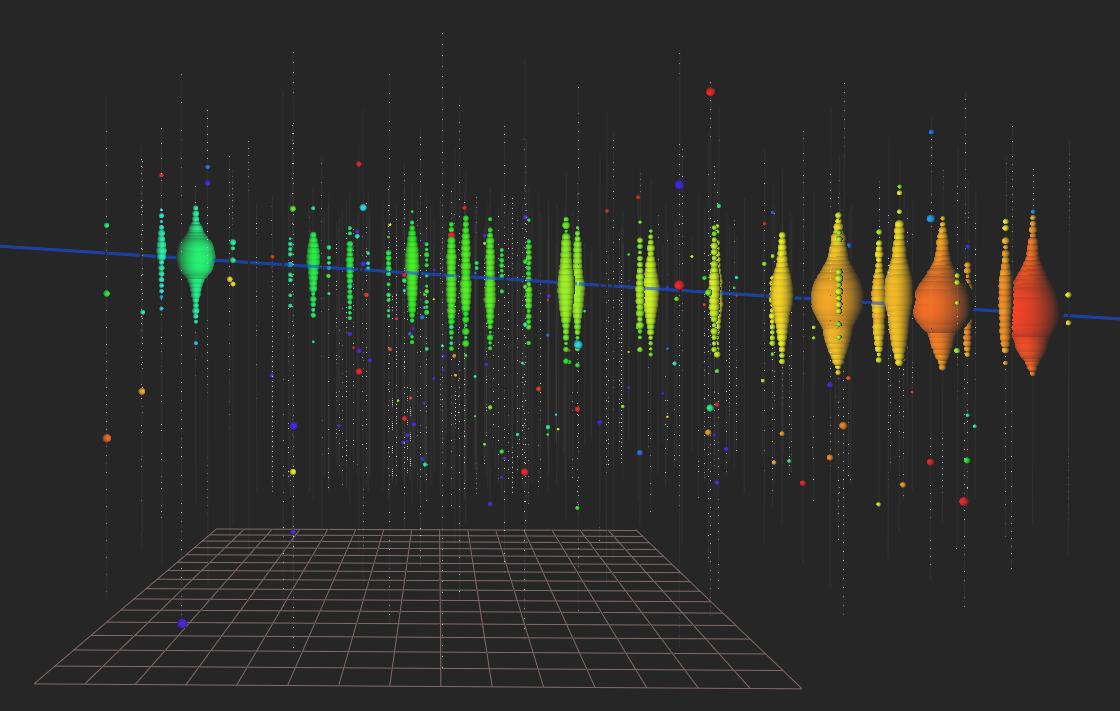
\includegraphics[width=0.9\textwidth]{images/Track.png}
                \credit{IceCube Collaboration}
            \end{figure}
        \end{column}
    \end{columns}
\end{frame}


\begin{frame}[c]
    \begin{columns}[onlytextwidth]
    \begin{column}{0.6\textwidth}
    \textbf{CORSIKA 8}
        \begin{itemize}
            \item CORSIKA~8: Newest version of the air shower simulation framework CORSIKA (currently under development)
            \begin{itemize}
                \item[$\rightarrow$] see: \url{gitlab.iap.kit.edu/AirShowerPhysics/corsika}
            \end{itemize}
            \item PROPOSAL is used in CORSIKA~8 as an electromagnetic and muonic shower model
            \begin{itemize}
                \item[$\rightarrow$] CORSIKA uses propagation steps provided by PROPOSAL modules
            \end{itemize}
        \end{itemize}

    \end{column}
        \begin{column}{0.4\textwidth}
            \begin{figure}
                \centering
                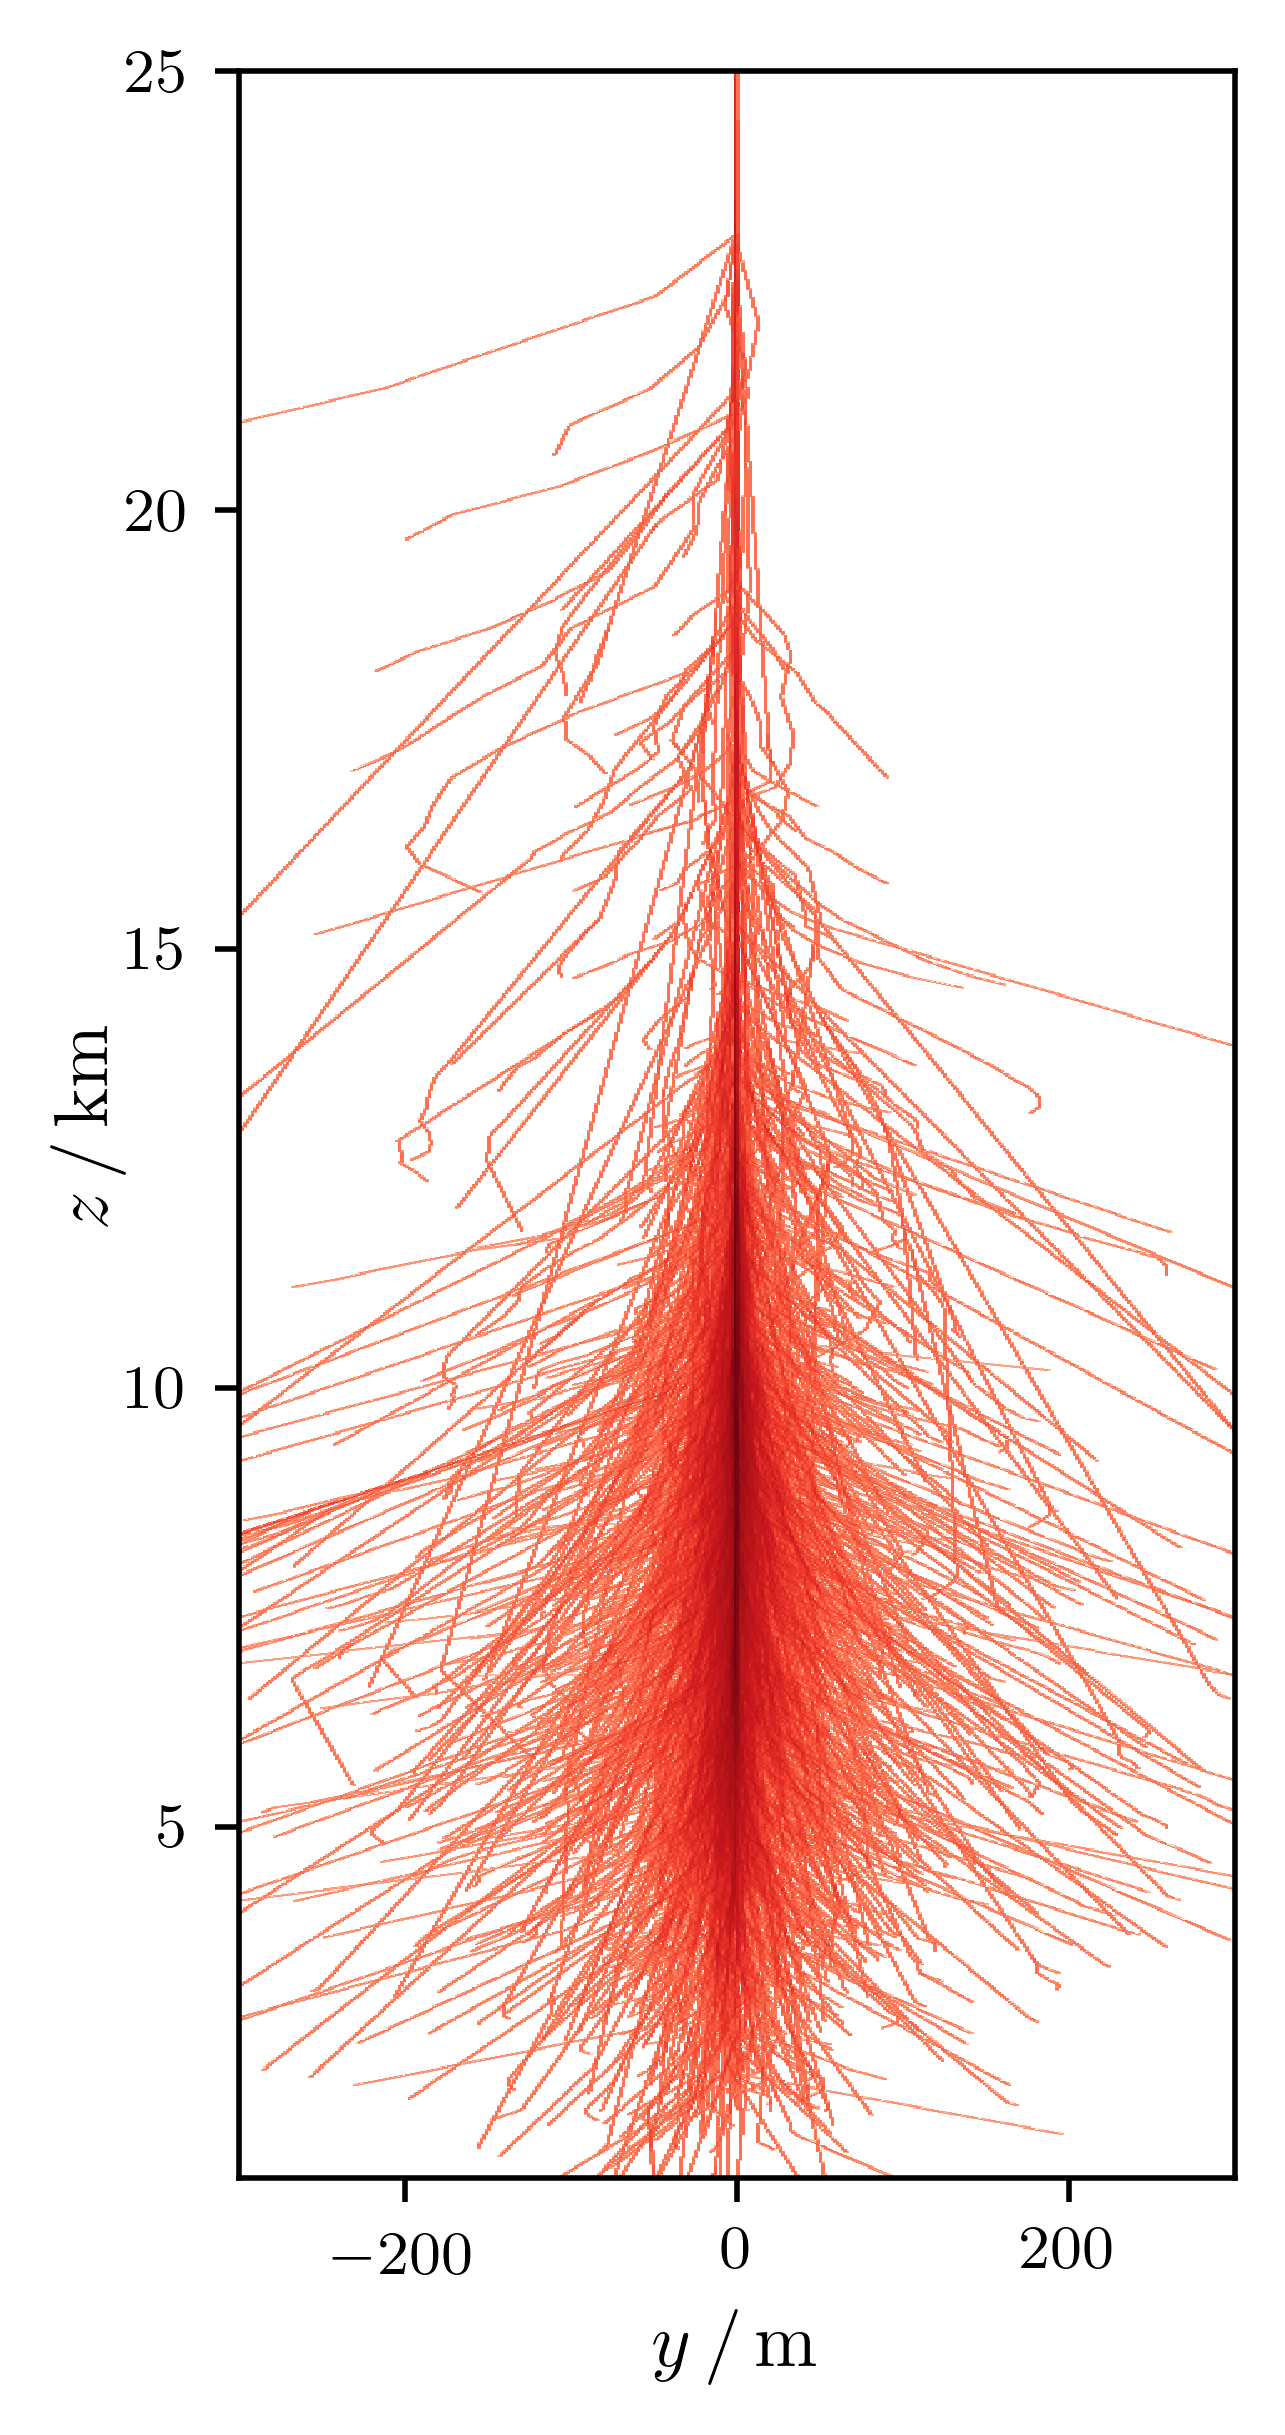
\includegraphics[width=0.6\textwidth]{plots/shower.png}
                \caption*{\SI{1}{\tera\electronvolt} $e^-$ shower simulated with CORSIKA 8}
            \end{figure}
        \end{column}
    \end{columns}
\end{frame}


\begin{frame}[c]
    \begin{figure}
        \centering
        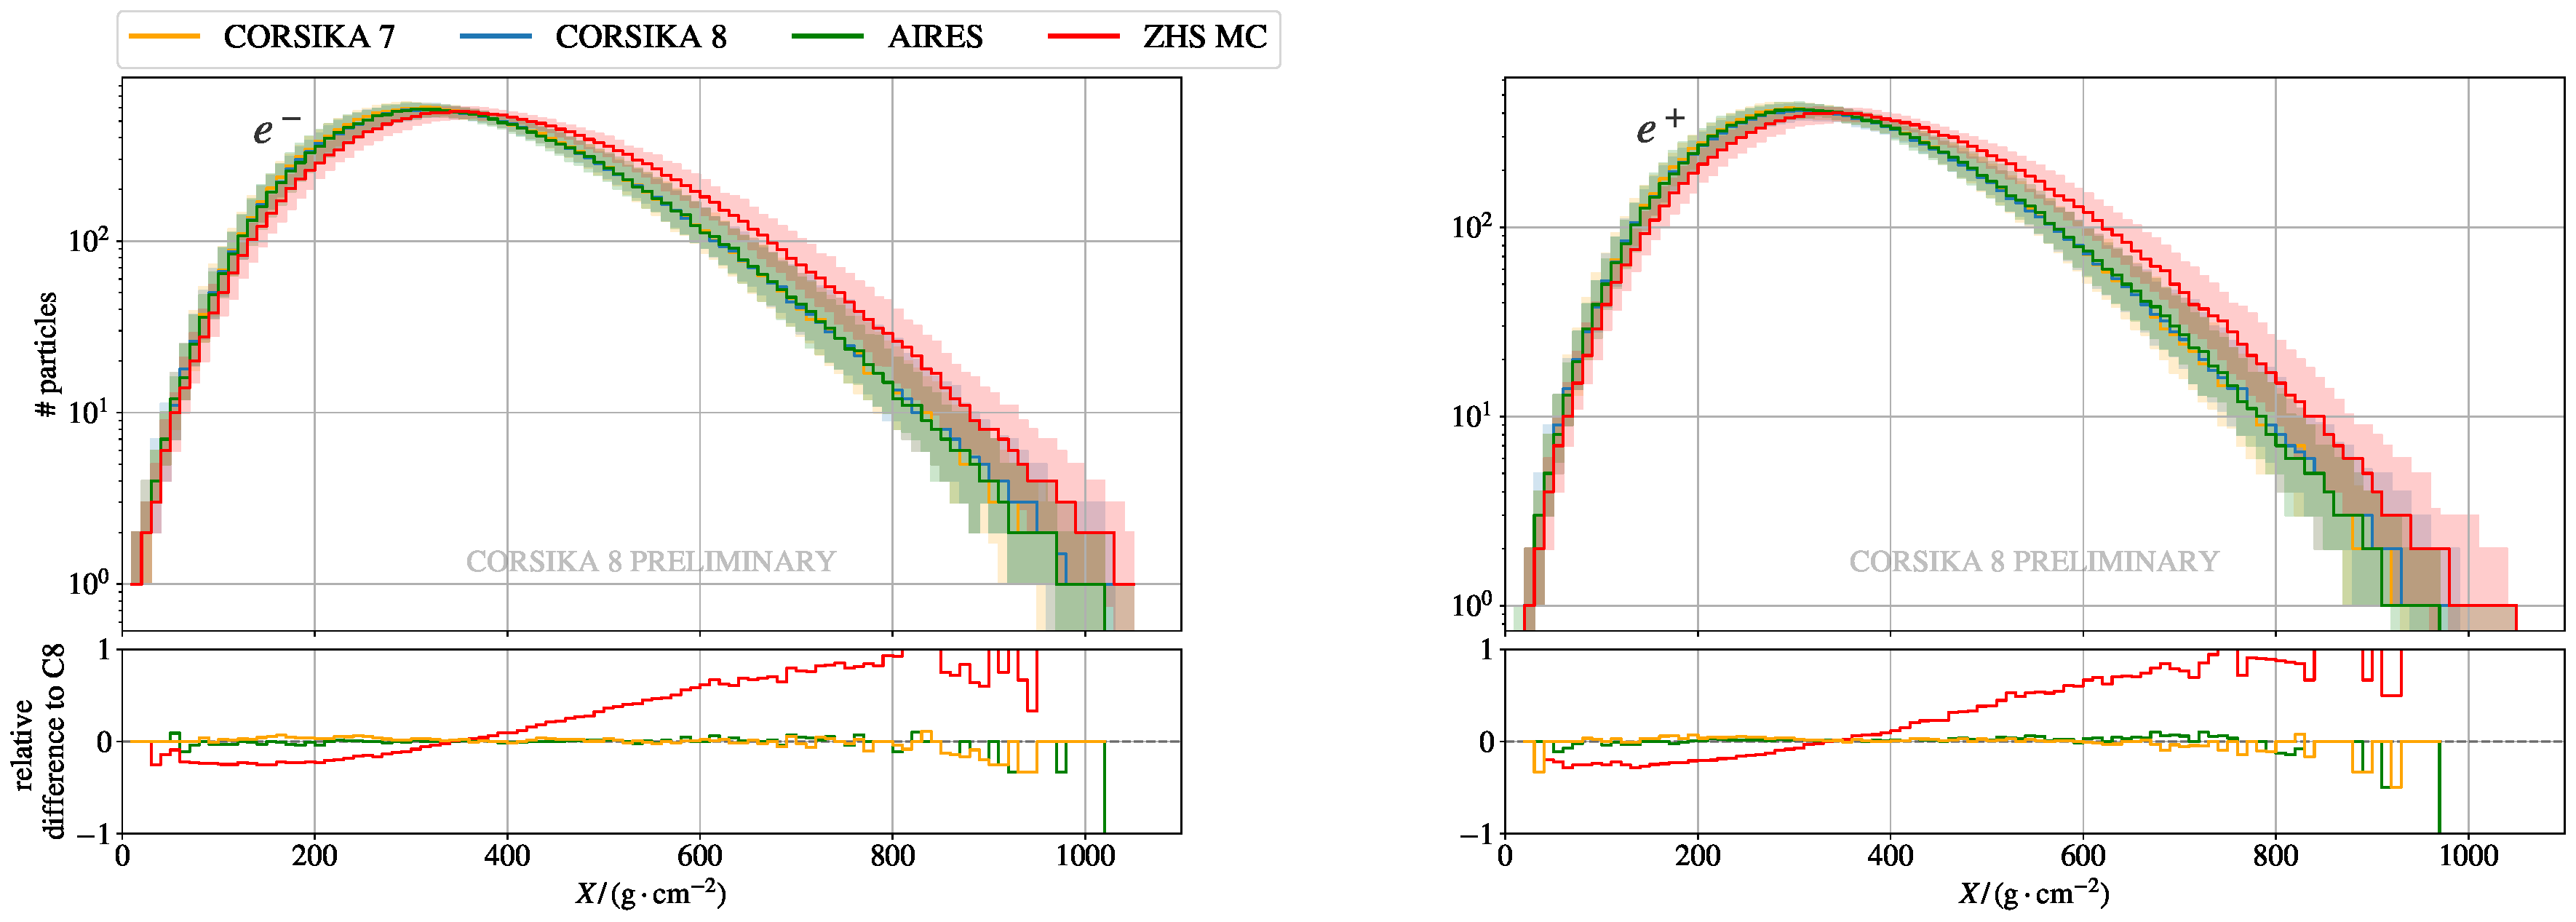
\includegraphics[width=0.85\textwidth]{plots/longitudinal_profile.pdf}
        \caption*{Longitudinal profile for 200 electromagnetic showers, initiated by \SI{1}{\tera\electronvolt} $e^-$}
    \end{figure}
    \begin{itemize}
        \item First comparisons of CORSIKA~8 results with other simulation frameworks are promising
    \end{itemize}

    \hspace{20pt} $\Rightarrow$ See \href{https://pos.sissa.it/395/428/}{PoS(ICRC2021)428}

\end{frame}



\begin{frame}[c]
    \begin{columns}[onlytextwidth]

    \begin{column}{0.5\textwidth}
        \textbf{Muography:}
        \begin{itemize}
            \item Non-invasive imaging technique using Cosmic Ray muons
            \begin{itemize}
                \item[$\rightarrow$] Trace muon number to observe density anomalies
            \end{itemize}
            \item PROPOSAL is a well-suited tool to provide the necessary muon simulations
            \begin{itemize}
                \item[$\rightarrow$] Currently analyzing the possibilities to use muography in mining with PROPOSAL simulations
            \end{itemize}
        \end{itemize}
    \end{column}

    \begin{column}{0.5\textwidth}
        \begin{figure}
            \begin{tikzpicture}[scale=0.85, every node/.style={scale=0.85}]
                \centering

                \coordinate (A) at (0, 0);

                % ground
                \draw[draw=none, fill=gray, fill opacity=1.0] ($ (A) + (-3.5,-2.5) $) rectangle ++(7, 5);

                % sky
                \draw[draw=none, fill={rgb:red,0.33;green,0.5;blue,0.98}, fill opacity=0.5] ($ (A) + (-3.5,2.5) $) rectangle ++(7, 1);
                \node[draw=none] at ($ (A) + (0.0, 3) $) {Sky};

                % mining shaft
                \draw[draw=none, fill={rgb:black,1;white,2}, fill opacity=1.0] ($ (A) + (2, -1.5) $) rectangle ++(0.25, 4.0);
                \draw[draw=none, fill={rgb:black,1;white,2}, fill opacity=1.0] ($ (A) + (-2.0, -1.5) $) rectangle ++(4, 0.5);

                \node[draw=none] at ($ (A) + (0.8, -1.25) $) {Mining shaft};

                % detector
                \node [cylinder, shape border rotate=90, draw,minimum height=0.40cm,minimum width=0.25cm, aspect=0.4] (detector) at ($ (A) + (-0.5, -1.3) $) {};

                % impurity
                \draw[draw=none,fill=black, fill opacity=0.7] ($ (A) + (0, 0.07) $) ellipse (0.3cm and 0.1cm);
                \node[draw=none, text width=1cm] at ($ (A) + (0.9, 0.07) $) {Anomaly};

                % muons
                \draw [densely dotted, blue, line width=0.25mm] ($ (A) + (-2.5, 3.0) $) -- ($ (detector) + (0.2, -0.5) $) node [near start, above, xshift=1ex] (TextNode) {$\mu$};

                \draw [densely dotted, blue, line width=0.25mm] ($ (A) + (-1.0, 3.0) $) -- ($ (detector) + (0.1, -0.5) $) node [near start, above, xshift=1ex] (TextNode) {$\mu$};

                \draw [densely dotted, blue, line width=0.25mm] ($ (A) + (1.0, 3.0) $) -- ($ (A) + (0, 0.07) $) node [pos=0.4, above, xshift=-1ex] (TextNode) {$\mu$};

            \end{tikzpicture}
        \end{figure}  
    \end{column}

    \end{columns}
\end{frame}

